\documentclass[aspectratio=169]{beamer}

\usepackage[utf8]{inputenc}
\usepackage[TS1,T1]{fontenc}
\usepackage{amsmath}
\usepackage{biblatex}
\usepackage{graphicx}
\usepackage{ctex}

\usepackage{tikz}
\usetikzlibrary{decorations.pathreplacing}

\addbibresource{references.bib} % Specify the bibliography file

\title{\Large{\bfseries{不定方程相关理论及其应用}}}
\date{\scriptsize{\today}}
\author{\small{\fangsong{郑欢誉}}}

\usetheme[language=english]{LTU}

\begin{document}
	
	\begin{frame}
		\titlepage
	\end{frame}
    
   	\begin{frame}{开题报告目录}{\small{Contents of Thesis Proposal}}
       \liwicki[1]{研究背景和意义\small{Research Background \& Significance}}\\
       \liwicki[2]{文献调研\small{Literature Research}}\\
       \liwicki[3]{研究方案和进度安排\small{Research Scheme \& Scheduling}}\\
   	\end{frame}
	
	\begin{frame}{研究背景和意义}{Research Background \& Significance}
		$$
        x^n + y^n = z^n
        $$
        \begin{quote}
            \begin{enumerate}
                \item[1637] Pierre de Fermat:提出猜想
                \vspace{5pt}
                \item[1839] $n=3, 4, 5, 7$,无穷递降
                \vspace{5pt}
                \item[1847] \textbf{Ernst Kummer:唯一分解,理想};
                %\vspace{2pt}
                $n$ \underline{正规素数}(不整除$\mathbb{Q}(\zeta_n)$的类数)
                \vspace{5pt}
                \item[1994] Andrew Wiles,模形式和椭圆曲线
            \end{enumerate}
        \end{quote}
	\end{frame}
	
	\begin{frame}{文献调研}{Literature Research}
    $$
    x^n+y^n=z^n \text{ no integer solution } (x, y, z) \text{ for } 2 < n
    $$
    \begin{flalign}
    \notag
    &\overset{analysis}{\implies} \text{ suffices to consider situation where } \underline{n=p \text{ odd prime}} \text{ \& } \underline{x,y,z \text{ coprime}}\\
    \notag
    &\overset{in \ \mathbb{Q}(\zeta_p)}{\implies} \underline{(x+y)(x+\zeta_p y)\cdots (x+\zeta_p^{p-1} y)=z^p} \Leftarrow \text{decomposition in } \mathbb{Z}[\zeta_p]
    \end{flalign}
	\end{frame}
    
    \begin{frame}{文献调研}{Literature Research}
    \begin{center}
    \textbf{"to what extend unique factorization fails or holds in number fields?"}
    \end{center}
    \liwicki[1]{factorization with respect to what subring? $\implies$ \underline{ring of integers}}\\
    \liwicki[2]{recovering unique factorization $\implies$ \underline{ideal}}\\
    \liwicki[3]{a way to measure by how much unique factorization fails? $\implies$ \underline{class number}}\\
    \liwicki[4]{simplifying how prime acts $\implies$ \underline{regular primes}}\\
    \liwicki[5]{the structure of the group of units in the ring of integers? $\implies$ \underline{unit theorem}}
    %\begin{enumerate}
    %\item \textit{factorization with respect to what subring?} $\implies$ \underline{ring of integers}
    %\item recovering unique factorization $\implies$ \underline{ideal}
    %\item \textit{a way to measure by how much unique factorization fails?} $\implies$ \underline{class number}
    %\item simplifying how prime acts $\implies$ \underline{regular primes}
    %\item \textit{the structure of the group of units in the ring of integers?} $\implies$ \underline{unit theorem}
    %\end{enumerate}
    \end{frame}
    
    \begin{frame}{文献调研}{Literature Research}
    Kummer: splits the problem (regular cases) into \\
    \begin{center}
    $x,y,z$ \underline{all coprime with $p$} v.s. \underline{exactly one divisible by $p$}
    \end{center}
    \begin{equation}
    \notag
    \begin{matrix}
        \prod_{i=0}^{p-1}\langle x+\zeta_p^iy\rangle = \langle z\rangle^p & \mid & \prod_{i=0}^{p-1}\langle x+\zeta_p^iy\rangle = I^{pm} \langle z_0\rangle^p
    \end{matrix}
    \end{equation}
    \end{frame}
    
    \begin{frame}{文献调研}{Literature Research}
    \textbf{FLT \& ABC conjecture}:\\
    \vspace{10pt}
    (ABC conjecture): $\forall \epsilon > 0$, $\exists$ constant $k_\epsilon$ s.t. for any coprime integers $a, b, c$ satisfying $a+b=c$,
    $$
    c \leq k_\epsilon \left(\prod_{p \ \text{prime}, \ p \mid abc} p\right)^{1+\epsilon}
    $$
    \begin{itemize}
    \item ABC $\implies$ FLT (Goldfeld, 1999)
    \item improvements on subexponential ABC (Hector, 2024)
    \end{itemize}
    \end{frame}
    
    \begin{frame}{文献调研}{Literature Research}
    \textbf{Asymptotic Fermat's Last Theorem}:\\
    \vspace{10pt}
    (Asymptotic FLT): $K$ a number field, there is a bound $B_K$, depending only on the field $K$, such that for all prime exponents $p > B_K$, there is no nontrivial solution to
    $$x^p + y^p + z^p = 0$$
    \begin{itemize}
    \item established the asymptotic Fermat's Last Theorem for many infinite families of number fields via \underline{class field theory} (Freitas, 2020)
    \end{itemize}
    \end{frame}
    
    \begin{frame}[fragile]{文献调研}{Literature Research}
    \textbf{Formalization} (Riccardo, 2024):\\
    \begin{figure}
 		\centering
 		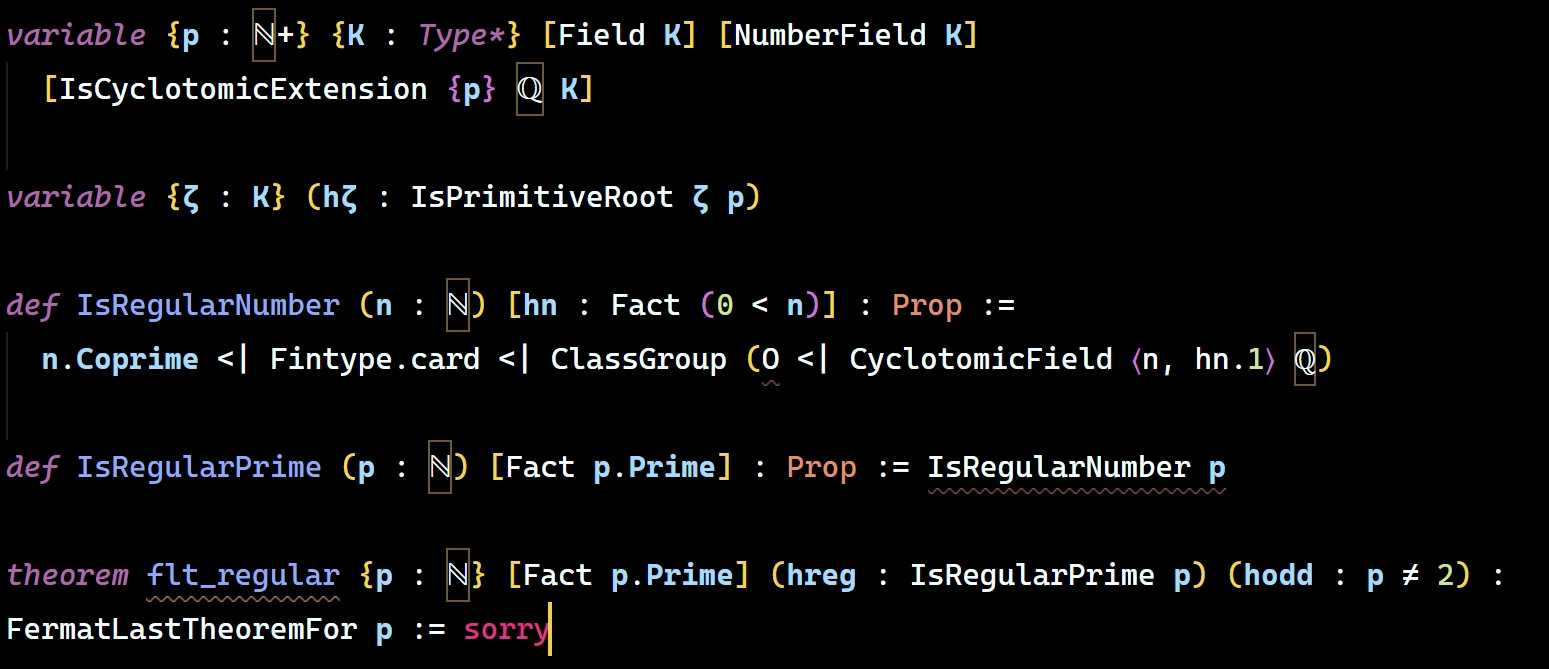
\includegraphics[width=0.8\linewidth]{screenshot.png}
	\end{figure}
    \end{frame}
	
	\begin{frame}{研究方案和进度安排}{Research Scheme \& Scheduling}
    \begin{quote}
            %\begin{small}
            \begin{itemize}
                \item[1-2月] 
                代数数论和交换代数(Ian\&Tall,Ash,Milne,Matsumura)\\
                \vspace{3pt}
                理解掌握Kummer关于正规素数情况的证明
                \vspace{10pt}
                \item[2-3月]
                通过Hector和Andrew的工作学习费马大定理与ABC猜想间的关联\\
                \vspace{3pt}
                利用类域论拓展性地了解渐进费马大定理
                \vspace{10pt}
                \item[3-4月] 形式化相关工作
            \end{itemize}
            %\end{small}
    \end{quote}
    \end{frame}
\end{document}